\documentclass[aspectratio=169]{beamer}

% ── Paket ────────────────────────────────────────────────────────────────────
\usepackage[utf8]{inputenc}
\usepackage[T1]{fontenc}
\usepackage{tikz}
\usepackage{pgfplots}
\pgfplotsset{compat=1.18}
\usepackage{booktabs}
\usepackage{array}
\usepackage{xcolor}
\usepackage{tcolorbox}
\tcbuselibrary{skins,breakable}

% Simple icon replacements (no fontawesome5 available)
\newcommand{\faChevronRight}{$\triangleright$}
\newcommand{\faCircle}{$\bullet$}
\newcommand{\faDatabase}{[DB]}
\newcommand{\faExclamationTriangle}{[!]}
\newcommand{\faChartLine}{[\char126]}
\newcommand{\faCheckCircle}{[\checkmark]}
\newcommand{\faTimesCircle}{[x]}
\newcommand{\faCalculator}{[\#]}
\newcommand{\faThumbsUp}{[+]}
\newcommand{\faThumbsDown}{[-]}
\newcommand{\faLink}{[L]}
\newcommand{\faStar}{[*]}
\newcommand{\faArrowDown}{[$\downarrow$]}
\newcommand{\faLightbulb}{[?]}
\newcommand{\faRocket}{[>>]}
\newcommand{\faChartBar}{[=]}
\newcommand{\faList}{[1]}
\newcommand{\faRobot}{[A]}
\newcommand{\faPalette}{[P]}
\newcommand{\faTag}{[\$]}
\newcommand{\faUsers}{[@]}
\newcommand{\faFlag}{[F]}
\newcommand{\faMapMarker}{[M]}
\newcommand{\faRoute}{[R]}
\newcommand{\faBrain}{[B]}
\newcommand{\faEnvelope}{[@]}

% ── Warna ─────────────────────────────────────────────────────────────────────
\definecolor{primary}{HTML}{1A3A5C}      % navy gelap
\definecolor{secondary}{HTML}{2E86AB}    % biru teal
\definecolor{accent}{HTML}{F4A261}       % oranye hangat
\definecolor{light}{HTML}{EFF6FB}        % biru sangat muda
\definecolor{darktext}{HTML}{1C1C1E}
\definecolor{mutedtext}{HTML}{6B7280}
\definecolor{success}{HTML}{27AE60}
\definecolor{danger}{HTML}{E74C3C}
\definecolor{warn}{HTML}{F39C12}

% ── Tema Beamer ───────────────────────────────────────────────────────────────
\usetheme{Madrid}
\usecolortheme[named=primary]{structure}
\setbeamercolor{palette primary}{bg=primary,fg=white}
\setbeamercolor{palette secondary}{bg=secondary,fg=white}
\setbeamercolor{palette tertiary}{bg=accent,fg=white}
\setbeamercolor{frametitle}{bg=primary,fg=white}
\setbeamercolor{title}{fg=white}
\setbeamercolor{subtitle}{fg=light}
\setbeamercolor{author}{fg=light}
\setbeamercolor{date}{fg=light}
\setbeamercolor{block title}{bg=secondary,fg=white}
\setbeamercolor{block body}{bg=light,fg=darktext}
\setbeamercolor{itemize item}{fg=accent}
\setbeamercolor{itemize subitem}{fg=secondary}
\setbeamertemplate{itemize item}{\small\faChevronRight}
\setbeamertemplate{itemize subitem}{\small\faCircle}
\setbeamertemplate{navigation symbols}{}
\setbeamerfont{frametitle}{size=\large,series=\bfseries}
\setbeamerfont{title}{size=\LARGE,series=\bfseries}

% ── Nomor halaman ─────────────────────────────────────────────────────────────
\setbeamertemplate{footline}{%
  \leavevmode%
  \hbox{%
    \begin{beamercolorbox}[wd=.33\paperwidth,ht=2.25ex,dp=1ex,center]{palette primary}%
      \usebeamerfont{author in head/foot}\insertshortauthor
    \end{beamercolorbox}%
    \begin{beamercolorbox}[wd=.34\paperwidth,ht=2.25ex,dp=1ex,center]{palette secondary}%
      \usebeamerfont{title in head/foot}\insertshorttitle
    \end{beamercolorbox}%
    \begin{beamercolorbox}[wd=.33\paperwidth,ht=2.25ex,dp=1ex,right]{palette tertiary}%
      \usebeamerfont{date in head/foot}\insertframenumber{}/\inserttotalframenumber\hspace*{2ex}
    \end{beamercolorbox}}%
  \vskip0pt%
}

% ── tcolorbox style ───────────────────────────────────────────────────────────
\tcbset{
  statbox/.style={
    colback=light, colframe=secondary, fonttitle=\bfseries,
    boxrule=1.5pt, arc=4pt, left=6pt, right=6pt, top=4pt, bottom=4pt
  },
  insightbox/.style={
    colback=accent!10, colframe=accent, fonttitle=\bfseries\color{darktext},
    boxrule=1.5pt, arc=4pt, left=6pt, right=6pt, top=4pt, bottom=4pt
  },
  implbox/.style={
    colback=secondary!10, colframe=secondary, fonttitle=\bfseries,
    boxrule=1.5pt, arc=4pt, left=6pt, right=6pt, top=4pt, bottom=4pt
  }
}

% ── Metadata ──────────────────────────────────────────────────────────────────
\title[MVP Riset Pasar -- Kelompok 12]{nechcode \\ Website Undangan Acara/Nikah Digital dan Gifting Site berbasis AI}
\subtitle{KBT -- Kelompok 12}
\author[Kelompok 12]{Louis C.S.L \and Hafidz Mulia \and Nabeel Farvez F \and M Rajwa Dzaki D \and Stanadyne Tolanda}
\date{2026}

% ══════════════════════════════════════════════════════════════════════════════
\begin{document}

%% ── TITLE SLIDE ──────────────────────────────────────────────────────────────
{
\setbeamertemplate{footline}{}
\begin{frame}[plain]
  \begin{tikzpicture}[remember picture,overlay]
    \fill[primary] (current page.north west) rectangle (current page.south east);
    \fill[secondary!60!primary,opacity=.35]
      (current page.north east) -- ++(-6,0) -- ++(0,-5) -- ++(6,0) -- cycle;
    \fill[accent,opacity=.18]
      (current page.south west) -- ++(5,0) -- ++(0,3.5) -- ++(-5,0) -- cycle;
    \node[anchor=center] at (current page.center) {%
      \begin{minipage}{0.82\paperwidth}
        \centering
        {\usebeamerfont{title}\usebeamercolor[fg]{title}\inserttitle\par}
        \vspace{0.4cm}
        {\usebeamerfont{subtitle}\usebeamercolor[fg]{subtitle}\insertsubtitle\par}
        \vspace{0.6cm}
        \textcolor{light!70}{\rule{0.5\textwidth}{0.4pt}}\par
        \vspace{0.4cm}
        {\small\color{light}
          \begin{tabular}{rl}
            5002221004 & Louis Cristiari S.L \\
            5002221022 & Hafidz Mulia \\
            5002221139 & Nabeel Farvez F \\
            5002221143 & M Rajwa Dzaki D \\
            5046231038 & Stanadyne Tolanda \\
          \end{tabular}\par}
        \vspace{0.2cm}
        {\small\color{light}\insertdate}
      \end{minipage}%
    };
  \end{tikzpicture}
\end{frame}
}

%% ── AGENDA ───────────────────────────────────────────────────────────────────
\begin{frame}{Outline}
  \begin{columns}[t]
    \column{0.48\textwidth}
      \begin{block}{Analisis}
        \begin{enumerate}\small
          \item Ringkasan Analisis
          \item Metodologi
          \item Rata-rata Skor Per Butir
          \item Perbandingan Dimensi Utama
        \end{enumerate}
      \end{block}
    \column{0.48\textwidth}
      \begin{block}{Temuan \& Rekomendasi}
        \begin{enumerate}\small\setcounter{enumi}{4}
          \item Top-2 vs Bottom-2 Box
          \item Funnel Ketertarikan \& Adopsi
          \item Driver Rekomendasi
          \item Rekomendasi Pengembangan MVP
        \end{enumerate}
      \end{block}
  \end{columns}
  \vspace{0.4cm}
  \begin{tcolorbox}[statbox, title={\faDatabase\quad Dataset}]
    \centering
    \textbf{15 responden} \quad|\quad Skala Likert 1--5 \quad|\quad Analisis: rata-rata, Top-2 box, Bottom-2 box
  \end{tcolorbox}
\end{frame}

%% ── RINGKASAN ANALISIS ───────────────────────────────────────────────────────
\begin{frame}{Ringkasan Analisis}
  \begin{columns}[T]
    \column{0.48\textwidth}
      \begin{tcolorbox}[statbox,title={\faExclamationTriangle\quad Masalah Terbesar}]
        \begin{itemize}\small
          \item \textbf{Tracking kehadiran tamu:} rata-rata \textcolor{accent}{\textbf{4.20}}
          \item \textbf{Kompleksitas mengundang banyak tamu:} rata-rata \textcolor{accent}{\textbf{4.07}}
        \end{itemize}
      \end{tcolorbox}
      \vspace{0.3cm}
      \begin{tcolorbox}[statbox,title={\faChartLine\quad Minat Solusi}]
        \begin{itemize}\small
          \item Fitur tracking absensi tamu:\par
            rata-rata \textcolor{success}{\textbf{4.60}} \quad Top-2 box \textcolor{success}{\textbf{93.3\%}}
        \end{itemize}
      \end{tcolorbox}
    \column{0.48\textwidth}
      \begin{tcolorbox}[insightbox,title={\faCheckCircle\quad Validasi MVP}]
        \begin{itemize}\small
          \item Produk membantu: \textbf{4.20}
          \item Mudah dipahami: \textbf{4.20}
          \item Nyaman digunakan: \textbf{4.07}
        \end{itemize}
      \end{tcolorbox}
      \vspace{0.3cm}
      \begin{tcolorbox}[implbox,title={\faTimesCircle\quad Area Perlu Perhatian}]
        \begin{itemize}\small
          \item \textbf{Sensitivitas harga:} pertimbangkan jika harga sesuai → hanya \textbf{3.60}
          \item \textbf{Produk perlu perbaikan:} \textbf{3.93}
        \end{itemize}
      \end{tcolorbox}
  \end{columns}
\end{frame}

%% ── METODOLOGI ───────────────────────────────────────────────────────────────
\begin{frame}{Metodologi}
  \begin{columns}[T]
    \column{0.32\textwidth}
      \begin{tcolorbox}[statbox,title={\faCalculator\quad 1. Rata-rata Skor},height=4.5cm]
        \small Melihat kecenderungan penilaian setiap butir pertanyaan pada skala 1--5.
      \end{tcolorbox}
    \column{0.32\textwidth}
      \begin{tcolorbox}[statbox,title={\faThumbsUp\quad 2. Top-2 Box},height=4.5cm]
        \small Persentase jawaban \textbf{4--5}. Mengukur tingkat persetujuan atau ketertarikan yang kuat.
      \end{tcolorbox}
    \column{0.32\textwidth}
      \begin{tcolorbox}[statbox,title={\faThumbsDown\quad 3. Bottom-2 Box},height=4.5cm]
        \small Persentase jawaban \textbf{1--2}. Mendeteksi area friksi atau penolakan dari responden.
      \end{tcolorbox}
  \end{columns}
  \vspace{0.4cm}
  \begin{tcolorbox}[insightbox,title={\faLink\quad Sumber Data}]
    \centering\small
    Wawancara + Google Form \textbullet{} 15 responden \textbullet{} Skala Likert 1--5
  \end{tcolorbox}
\end{frame}

%% ── GRAFIK 1: RATA-RATA SKOR ─────────────────────────────────────────────────
\begin{frame}{Grafik 1 -- Rata-rata Skor Per Butir Pertanyaan}
\centering
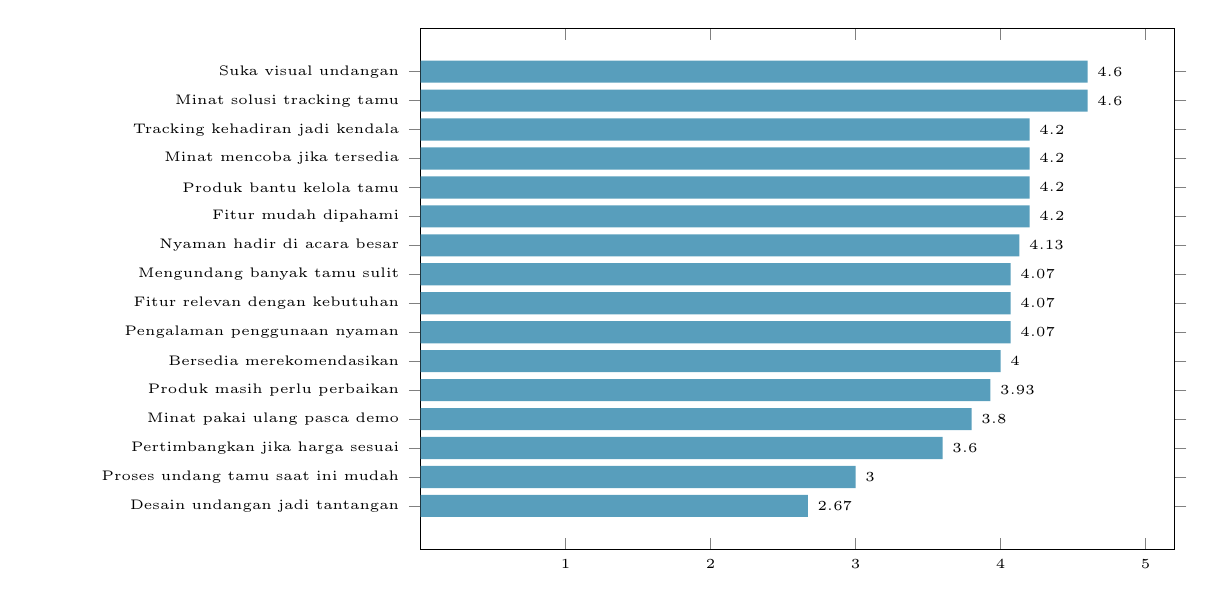
\begin{tikzpicture}
\begin{axis}[
  xbar,
  width=0.92\textwidth, height=8.2cm,
  xmin=0, xmax=5.2,
  bar width=8pt,
  symbolic y coords={
    {Desain undangan jadi tantangan},
    {Proses undang tamu saat ini mudah},
    {Pertimbangkan jika harga sesuai},
    {Minat pakai ulang pasca demo},
    {Produk masih perlu perbaikan},
    {Bersedia merekomendasikan},
    {Pengalaman penggunaan nyaman},
    {Fitur relevan dengan kebutuhan},
    {Mengundang banyak tamu sulit},
    {Nyaman hadir di acara besar},
    {Fitur mudah dipahami},
    {Produk bantu kelola tamu},
    {Minat mencoba jika tersedia},
    {Tracking kehadiran jadi kendala},
    {Minat solusi tracking tamu},
    {Suka visual undangan}
  },
  ytick=data,
  yticklabel style={font=\tiny,align=right,text width=4.6cm},
  xtick={1,2,3,4,5},
  nodes near coords,
  nodes near coords style={font=\tiny, /pgf/number format/.cd, fixed, precision=2},
  every axis/.append style={font=\tiny},
  title style={font=\small\bfseries},
]
\addplot[fill=secondary!80, draw=none] coordinates {
  (2.67,{Desain undangan jadi tantangan})
  (3.00,{Proses undang tamu saat ini mudah})
  (3.60,{Pertimbangkan jika harga sesuai})
  (3.80,{Minat pakai ulang pasca demo})
  (3.93,{Produk masih perlu perbaikan})
  (4.00,{Bersedia merekomendasikan})
  (4.07,{Pengalaman penggunaan nyaman})
  (4.07,{Fitur relevan dengan kebutuhan})
  (4.07,{Mengundang banyak tamu sulit})
  (4.13,{Nyaman hadir di acara besar})
  (4.20,{Fitur mudah dipahami})
  (4.20,{Produk bantu kelola tamu})
  (4.20,{Minat mencoba jika tersedia})
  (4.20,{Tracking kehadiran jadi kendala})
  (4.60,{Minat solusi tracking tamu})
  (4.60,{Suka visual undangan})
};
\end{axis}
\end{tikzpicture}
\end{frame}

%% ── INSIGHT GRAFIK 1 ─────────────────────────────────────────────────────────
\begin{frame}{Insight -- Rata-rata Skor}
  \begin{columns}[T]
    \column{0.48\textwidth}
      \begin{tcolorbox}[insightbox,title={\faStar\quad Skor Tertinggi}]
        \begin{itemize}\small
          \item \textbf{Suka visual undangan menarik:} \textcolor{accent}{\textbf{4.60}}
          \item \textbf{Tertarik solusi tracking absensi:} \textcolor{accent}{\textbf{4.60}}
        \end{itemize}
        \vspace{0.2cm}
        \small Kebutuhan pasar bukan hanya fungsi administratif, tetapi juga \textit{kualitas presentasi} undangan.
      \end{tcolorbox}
    \column{0.48\textwidth}
      \begin{tcolorbox}[statbox,title={\faArrowDown\quad Skor Terendah}]
        \begin{itemize}\small
          \item \textbf{Desain undangan jadi tantangan:} \textcolor{danger}{\textbf{2.67}}
          \item \textbf{Proses mengundang saat ini mudah:} \textbf{3.00}
        \end{itemize}
        \vspace{0.2cm}
        \small Desain bukan pain point paling universal; alur mengundang belum sepenuhnya efisien.
      \end{tcolorbox}
  \end{columns}
  \vspace{0.3cm}
  \begin{tcolorbox}[implbox,title={\faLightbulb\quad Implikasi Produk}]
    \small Posisikan produk sebagai \textbf{solusi operasional + presentasi visual}.
    Tonjolkan nilai estetika undangan seiring fitur RSVP/absensi.
  \end{tcolorbox}
\end{frame}

%% ── GRAFIK 2: DIMENSI UTAMA ──────────────────────────────────────────────────
\begin{frame}{Grafik 2 -- Perbandingan Dimensi Utama}
  \begin{columns}[T]
    \column{0.52\textwidth}
      \vspace{0.5cm}
      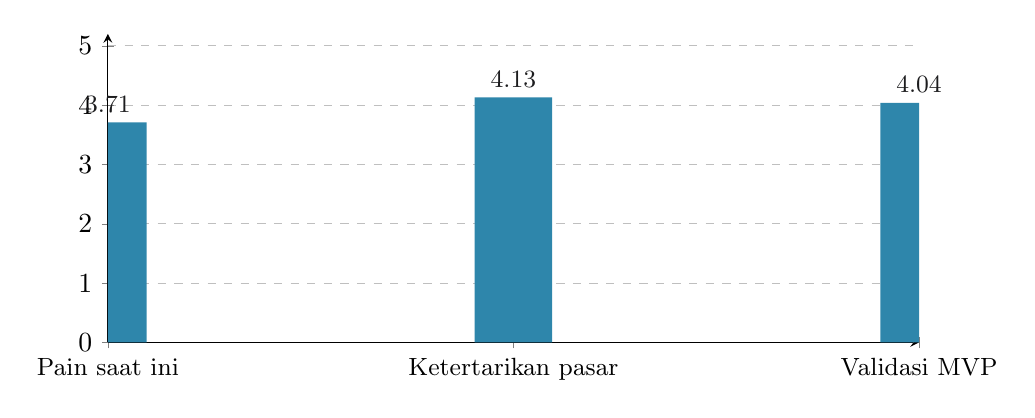
\begin{tikzpicture}
        \begin{axis}[
          ybar,
          width=0.98\linewidth,
          height=5.5cm,
          bar width=28pt,
          ymin=0, ymax=5.2,
          symbolic x coords={{Pain saat ini},{Ketertarikan pasar},{Validasi MVP}},
          xtick=data,
          xticklabel style={font=\small},
          ytick={0,1,2,3,4,5},
          nodes near coords,
          nodes near coords style={font=\small\bfseries,color=darktext},
          /pgf/number format/.cd, fixed, precision=2,
          axis x line=bottom, axis y line=left,
          ymajorgrids=true, grid style=dashed,
        ]
        \addplot[fill=secondary,draw=none] coordinates {
          ({Pain saat ini},3.71)
          ({Ketertarikan pasar},4.13)
          ({Validasi MVP},4.04)
        };
        \end{axis}
      \end{tikzpicture}
    \column{0.46\textwidth}
      \vspace{0.6cm}
      \begin{tcolorbox}[insightbox,title={\faLightbulb\quad Insight}]
        \small\textbf{Ketertarikan pasar} (4.13) \& \textbf{Validasi MVP} (4.04) lebih tinggi dari \textbf{Pain saat ini} (3.71).\\[4pt]
        Pasar sudah siap menerima solusi dan MVP berhasil menjelaskan \textit{value proposition} dasarnya.
      \end{tcolorbox}
      \vspace{0.3cm}
      \begin{tcolorbox}[implbox,title={\faRocket\quad Implikasi}]
        \small Fokus berikutnya: \textbf{bukan} membuktikan kebutuhan (sudah jelas), melainkan meningkatkan kualitas pengalaman produk untuk mendorong \textit{reuse}, rekomendasi, dan \textit{willingness to pay}.
      \end{tcolorbox}
  \end{columns}
\end{frame}

%% ── GRAFIK 3: TOP-2 vs BOTTOM-2 BOX ─────────────────────────────────────────
\begin{frame}{Grafik 3 -- Top-2 Box vs Bottom-2 Box (Area Penting)}
\centering
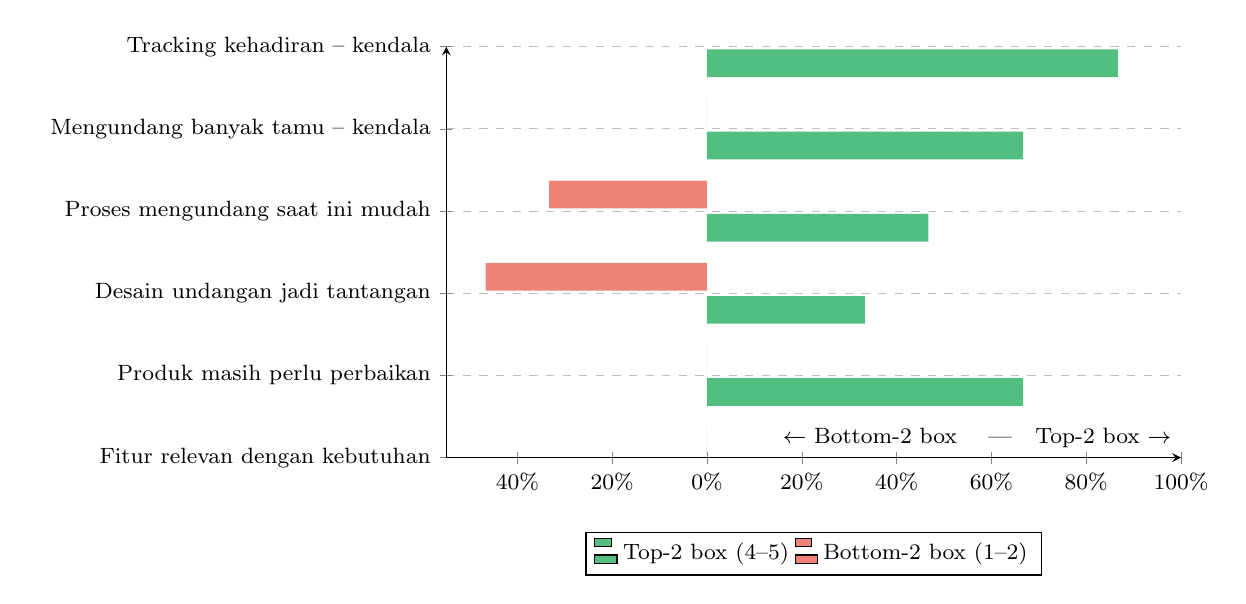
\begin{tikzpicture}
\begin{axis}[
  xbar,
  width=0.90\textwidth, height=6.8cm,
  xmin=-55, xmax=100,
  bar width=10pt,
  symbolic y coords={
    {Fitur relevan dengan kebutuhan},
    {Produk masih perlu perbaikan},
    {Desain undangan jadi tantangan},
    {Proses mengundang saat ini mudah},
    {Mengundang banyak tamu -- kendala},
    {Tracking kehadiran -- kendala}
  },
  ytick=data,
  yticklabel style={font=\footnotesize,align=right,text width=5cm},
  xtick={-40,-20,0,20,40,60,80,100},
  xticklabels={40\%,20\%,0\%,20\%,40\%,60\%,80\%,100\%},
  axis x line=center, axis y line=left,
  xlabel={\footnotesize $\leftarrow$ Bottom-2 box \quad|\quad Top-2 box $\rightarrow$},
  legend style={at={(0.5,-0.18)},anchor=north,legend columns=2},
  ymajorgrids=true, grid style=dashed,
  every axis/.append style={font=\footnotesize},
]
% Top-2 box (positif)
\addplot[fill=success!80,draw=none,xbar] coordinates {
  (60,{Fitur relevan dengan kebutuhan})
  (66.7,{Produk masih perlu perbaikan})
  (33.3,{Desain undangan jadi tantangan})
  (46.7,{Proses mengundang saat ini mudah})
  (66.7,{Mengundang banyak tamu -- kendala})
  (86.7,{Tracking kehadiran -- kendala})
};
% Bottom-2 box (negatif -- dibalik ke kiri)
\addplot[fill=danger!70,draw=none,xbar] coordinates {
  (-0,{Fitur relevan dengan kebutuhan})
  (-0,{Produk masih perlu perbaikan})
  (-46.7,{Desain undangan jadi tantangan})
  (-33.3,{Proses mengundang saat ini mudah})
  (-0,{Mengundang banyak tamu -- kendala})
  (-13.3,{Tracking kehadiran -- kendala})
};
\legend{Top-2 box (4--5), Bottom-2 box (1--2)}
\end{axis}
\end{tikzpicture}
\end{frame}

%% ── INSIGHT GRAFIK 3 ─────────────────────────────────────────────────────────
\begin{frame}{Insight -- Top-2 Box vs Bottom-2 Box}
  \begin{tcolorbox}[insightbox,title={\faChartBar\quad Temuan Kunci}]
    \begin{itemize}\small
      \item \textbf{Tracking kehadiran tamu:} Top-2 box \textcolor{success}{\textbf{86.7\%}} -- sinyal sangat kuat sebagai \textit{core feature}
      \item \textbf{Desain undangan jadi tantangan:} Top-2 box hanya 33.3\%, Bottom-2 box \textcolor{danger}{46.7\%} -- bukan pain point universal
      \item \textbf{Produk masih perlu perbaikan:} Top-2 box \textbf{66.7\%} -- mayoritas melihat ruang improvement yang nyata
    \end{itemize}
  \end{tcolorbox}
  \vspace{0.3cm}
  \begin{columns}[T]
    \column{0.32\textwidth}
      \begin{tcolorbox}[statbox,title={\faList\quad 1. Core First},height=3.2cm]
        \tiny RSVP, check-in, dashboard kehadiran, notifikasi, status real-time
      \end{tcolorbox}
    \column{0.32\textwidth}
      \begin{tcolorbox}[statbox,title={\faRobot\quad 2. Automation},height=3.2cm]
        \tiny Import kontak, broadcast undangan, reminder otomatis, pengelompokan tamu
      \end{tcolorbox}
    \column{0.32\textwidth}
      \begin{tcolorbox}[statbox,title={\faPalette\quad 3. Design},height=3.2cm]
        \tiny Template visual yang baik, bukan editor kompleks pada fase MVP berikutnya
      \end{tcolorbox}
  \end{columns}
\end{frame}

%% ── GRAFIK 4: FUNNEL ─────────────────────────────────────────────────────────
\begin{frame}{Grafik 4 -- Funnel Ketertarikan \& Adopsi}
  \begin{columns}[T]
    \column{0.52\textwidth}
    \vspace{0.3cm}
    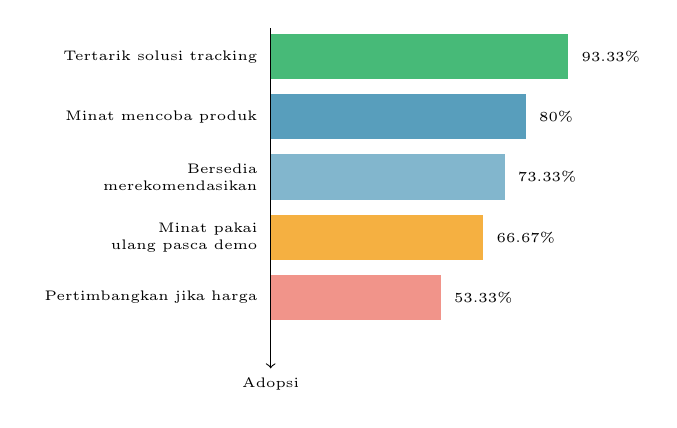
\begin{tikzpicture}[scale=0.90]
      % Funnel bars (trapezoid shapes via TikZ)
      \def\labels{{"Tertarik solusi tracking","Minat mencoba produk","Bersedia merekomendasikan","Minat pakai ulang pasca demo","Pertimbangkan jika harga sesuai"}}
      \def\vals{{93.33,80,73.33,66.67,53.33}}
      \def\clrs{{"success!85","secondary!80","secondary!60","warn!80","danger!60"}}
      % Draw horizontal bars
      \foreach \i/\val/\lbl/\clr in {
        0/93.33/{Tertarik solusi tracking}/success!85,
        1/80/{Minat mencoba produk}/secondary!80,
        2/73.33/{Bersedia merekomendasikan}/secondary!60,
        3/66.67/{Minat pakai ulang pasca demo}/warn!80,
        4/53.33/{Pertimbangkan jika harga}/danger!60%
      }{
        \pgfmathsetmacro\y{4.2-\i*0.85}
        \pgfmathsetmacro\w{\val*0.045}
        \fill[\clr] (0,\y-0.32) rectangle (\w,\y+0.32);
        \node[right,font=\tiny] at (\w+0.05,\y) {\val\%};
        \node[left,font=\tiny,align=right,text width=2.8cm] at (-0.05,\y) {\lbl};
      }
      \draw[->] (0,4.6) -- (0,-0.2) node[below,font=\tiny]{Adopsi};
    \end{tikzpicture}

    \column{0.46\textwidth}
      \vspace{0.3cm}
      \begin{tcolorbox}[insightbox,title={\faLightbulb\quad Insight Funnel}]
        \small Penurunan tajam pada harga (53.3\%) setelah minat awal tinggi (93.3\%). Setelah itu minat \textit{reuse} naik (80\%), mengindikasikan \textbf{value proposition kuat} namun hambatan di pricing dan kematangan experience.
      \end{tcolorbox}
      \vspace{0.3cm}
      \begin{tcolorbox}[implbox,title={\faTag\quad Implikasi Bisnis}]
        \begin{itemize}\tiny
          \item \textbf{Paket entry-level/freemium} untuk event kecil
          \item \textbf{Komunikasi ROI:} hemat waktu admin, akurasi hadir
          \item \textbf{Perbaikan onboarding} agar \textit{reuse} konsisten meningkat
        \end{itemize}
      \end{tcolorbox}
  \end{columns}
\end{frame}

%% ── GRAFIK 5: DRIVER REKOMENDASI ─────────────────────────────────────────────
\begin{frame}{Grafik 5 -- Driver Kemauan Merekomendasikan Produk}
  \begin{columns}[T]
    \column{0.52\textwidth}
    \vspace{0.3cm}
    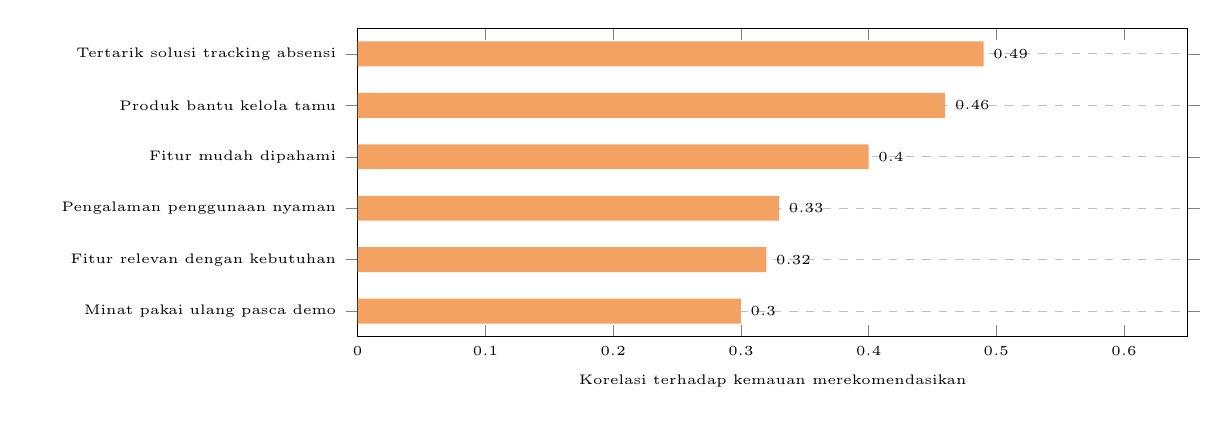
\begin{tikzpicture}
    \begin{axis}[
      xbar,
      width=\linewidth,
      height=5.5cm,
      bar width=9pt,
      xmin=0, xmax=0.65,
      xtick={0,0.1,0.2,0.3,0.4,0.5,0.6},
      xticklabel style={font=\tiny},
      symbolic y coords={
        {Minat pakai ulang pasca demo},
        {Fitur relevan dengan kebutuhan},
        {Pengalaman penggunaan nyaman},
        {Fitur mudah dipahami},
        {Produk bantu kelola tamu},
        {Tertarik solusi tracking absensi}
      },
      ytick=data,
      yticklabel style={font=\tiny,align=right,text width=3.8cm},
      nodes near coords,
      nodes near coords style={font=\tiny},
      /pgf/number format/.cd, fixed, precision=2,
      ymajorgrids=true, grid style=dashed,
      xlabel={\tiny Korelasi terhadap kemauan merekomendasikan},
    ]
    \addplot[fill=accent,draw=none] coordinates {
      (0.30,{Minat pakai ulang pasca demo})
      (0.32,{Fitur relevan dengan kebutuhan})
      (0.33,{Pengalaman penggunaan nyaman})
      (0.40,{Fitur mudah dipahami})
      (0.46,{Produk bantu kelola tamu})
      (0.49,{Tertarik solusi tracking absensi})
    };
    \end{axis}
    \end{tikzpicture}

    \column{0.46\textwidth}
      \vspace{0.3cm}
      \begin{tcolorbox}[insightbox,title={\faStar\quad Top 3 Driver}]
        \begin{enumerate}\small
          \item Ketertarikan pada solusi tracking \textbf{(r=0.49)}
          \item Persepsi produk membantu \textbf{(r=0.46)}
          \item Kemudahan memahami fitur \textbf{(r=0.40)}
        \end{enumerate}
      \end{tcolorbox}
      \vspace{0.3cm}
      \begin{tcolorbox}[implbox,title={\faUsers\quad Implikasi}]
        \begin{itemize}\tiny
          \item \textbf{Kejelasan manfaat} sejak awal: demo, empty state edukatif
          \item \textbf{Simplicity of use:} buat event $\to$ impor tamu $\to$ kirim $\to$ pantau
          \item \textbf{Proof of value:} dashboard ringkas status RSVP real-time
        \end{itemize}
      \end{tcolorbox}
  \end{columns}
\end{frame}

%% ── TABEL STATISTIK ──────────────────────────────────────────────────────────
\begin{frame}{Tabel Ringkasan Statistik}
\centering
\footnotesize
\setlength{\tabcolsep}{4pt}
\begin{tabular}{@{}lccc@{}}
\toprule
\textbf{Butir Pertanyaan} & \textbf{Rata-rata} & \textbf{Top-2} & \textbf{Bot-2} \\
\midrule
Menyukai undangan visual menarik        & 4.60 & \textcolor{success}{100.0\%} & 0.0\% \\
Tertarik solusi tracking absensi tamu   & 4.60 & \textcolor{success}{93.3\%}  & 0.0\% \\
Tracking kehadiran tamu -- kendala      & 4.20 & \textcolor{success}{86.7\%}  & 13.3\% \\
Tertarik mencoba produk jika tersedia   & 4.20 & 80.0\% & 0.0\% \\
Produk membantu mengelola tamu          & 4.20 & \textcolor{success}{86.7\%}  & 0.0\% \\
Fitur dan cara kerja mudah dipahami     & 4.20 & 80.0\% & 0.0\% \\
Nyaman hadir di acara besar             & 4.13 & 80.0\% & 0.0\% \\
Mengundang banyak tamu -- kendala       & 4.07 & 66.7\% & 0.0\% \\
Fitur produk relevan dengan kebutuhan   & 4.07 & 60.0\% & 0.0\% \\
Pengalaman penggunaan cukup nyaman      & 4.07 & 80.0\% & 0.0\% \\
Bersedia merekomendasikan               & 4.00 & 73.3\% & 6.7\% \\
Produk masih perlu perbaikan            & 3.93 & 66.7\% & 0.0\% \\
Tertarik menggunakan kembali pasca demo & 3.80 & 66.7\% & 13.3\% \\
Pertimbangkan jika harga sesuai         & 3.60 & 53.3\% & \textcolor{danger}{20.0\%} \\
Proses mengundang tamu saat ini mudah   & 3.00 & 46.7\% & \textcolor{danger}{33.3\%} \\
Desain undangan menjadi tantangan       & 2.67 & 33.3\% & \textcolor{danger}{46.7\%} \\
\bottomrule
\end{tabular}
\end{frame}

%% ── REKOMENDASI MVP ──────────────────────────────────────────────────────────
\begin{frame}{Rekomendasi Pengembangan Produk MVP}
  \begin{columns}[T]
    \column{0.48\textwidth}
      \begin{tcolorbox}[statbox,title={\quad 1. Core: Tracking Tamu}]
        \tiny RSVP, check-in, dashboard kehadiran, reminder, update status real-time
      \end{tcolorbox}
      \vspace{0.15cm}
      \begin{tcolorbox}[statbox,title={\quad 2. Sederhanakan Alur}]
        \tiny Buat acara $\to$ tambah/impor tamu $\to$ kirim undangan $\to$ pantau RSVP/kehadiran
      \end{tcolorbox}
      \vspace{0.15cm}
      \begin{tcolorbox}[statbox,title={\quad 3. Onboarding \& Kejelasan}]
        \tiny UX writing, empty state edukatif, tooltip, demo, template onboarding
      \end{tcolorbox}
    \column{0.48\textwidth}
      \begin{tcolorbox}[insightbox,title={\quad 4. Strategi Harga}]
        \tiny Paket gratis terbatas, paket per event, atau tier berdasarkan jumlah tamu dan kebutuhan tracking
      \end{tcolorbox}
      \vspace{0.15cm}
      \begin{tcolorbox}[insightbox,title={\quad 5. Visual sebagai Diferensiasi}]
        \tiny Pertahankan kualitas template agar produk terasa \textit{premium} sejak interaksi pertama
      \end{tcolorbox}
      \vspace{0.15cm}
      \begin{tcolorbox}[implbox,title={\quad Prioritas Roadmap}]
        \tiny \textbf{Core ops} $\to$ \textbf{Automation} $\to$ \textbf{Design differentiation}
      \end{tcolorbox}
  \end{columns}
\end{frame}

%% ── KESIMPULAN / PENUTUP ─────────────────────────────────────────────────────
{
\setbeamertemplate{footline}{}
\begin{frame}[plain]
  \begin{tikzpicture}[remember picture,overlay]
    \fill[primary] (current page.north west) rectangle (current page.south east);
    \fill[secondary!50,opacity=.3]
      (current page.south east) -- ++(-5,0) -- ++(0,4) -- ++(5,0) -- cycle;
  \end{tikzpicture}
  \vspace{1cm}
  \begin{center}
    {\Large\bfseries\color{white} Kesimpulan}\par
    \vspace{0.6cm}
    \begin{beamercolorbox}[center,wd=0.88\textwidth,rounded=true,shadow=true]{block body}
      \vspace{0.3cm}
      \small MVP sudah menunjukkan \textbf{product signal positif}: pasar tertarik, manfaat dirasakan,
      dan ada potensi advokasi. Tantangan berikutnya bukan membuktikan kebutuhan, melainkan
      \textbf{mematangkan pengalaman produk} dan \textbf{strategi monetisasi}.\\[6pt]
      Dengan fokus pada \textit{tracking tamu, simplifikasi alur, onboarding,} dan \textit{pricing},
      peluang meningkatkan \textit{reuse}, rekomendasi, dan konversi ke penggunaan nyata akan
      jauh lebih besar.
      \vspace{0.3cm}
    \end{beamercolorbox}
    \vspace{0.7cm}
    {\color{light}\rule{0.5\textwidth}{0.4pt}}\par
    \vspace{0.4cm}
    {\color{light}\small \faEnvelope\quad Kelompok 12 -- KBT 2026}\par
  \end{center}
\end{frame}
}

\end{document}